\begin{figure}[t]
\centering
\subfigure[Graph mit zufälliger Ordnung]{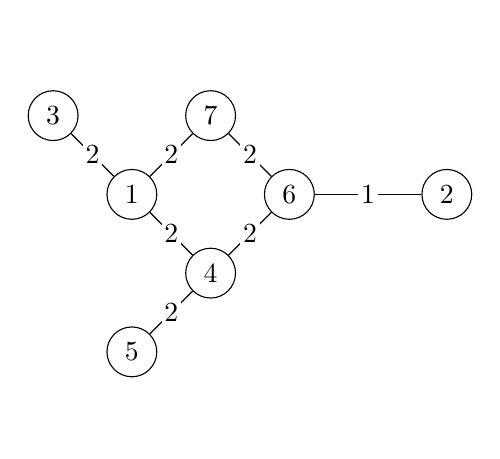
\begin{tikzpicture}
  \fill [white] (-3, -3) rectangle (2, 2) node {};  % Zentriere Graph.
  \tikzstyle{node}=[circle,draw, minimum width=18pt, inner sep=0pt, fill=white]
  \tikzstyle{label}=[fill=white, inner sep=1pt]

  \node[node] (1) at (-3, 1)  {$3$};
  \node[node] (2) at (-2, 0)  {$1$};
  \node[node] (3) at (-1, 1)  {$7$};
  \node[node] (4) at (-1, -1) {$4$};
  \node[node] (5) at (0, 0)   {$6$};
  \node[node] (6) at (-2, -2) {$5$};
  \node[node] (7) at (2, 0)   {$2$};

  \path (1) edge node[label] {$2$} (2);
  \path (2) edge node[label] {$2$} (3);
  \path (2) edge node[label] {$2$} (4);
  \path (3) edge node[label] {$2$} (5);
  \path (4) edge node[label] {$2$} (5);
  \path (4) edge node[label] {$2$} (6);
  \path (5) edge node[label] {$1$} (7);
\end{tikzpicture}
}
\hspace{1cm}
\subfigure[Bestimmung des Normalized-Cuts]{\begin{tabular}[b]{ccc}
  \toprule
  Kante & Gewicht & Normalized-Cut\\
  \toprule
  $\left(1,3\right)$ & 2 & $\mathbf{1.\overline{3}}\,\,\,$\\
  $\left(1,4\right)$ & 2 & $0.\overline{3}\,\,\,$\\
  $\left(1,7\right)$ & 2 & $0.8\overline{3}$\\
  \midrule
  $\left(2,6\right)$ & $1$ & $\mathbf{1.2}\,\,\,$\\
  \midrule
  $\left(4,5\right)$ & $2$ & $\mathbf{1.\overline{3}}\,\,\,$\\
  $\left(4,6\right)$ & $2$ & $0.7\overline{3}$\\
  \midrule
  $\left(6,7\right)$ & $2$ & $\mathbf{0.9}\,\,\,$\\
  \bottomrule
\end{tabular}
}
\hspace{1cm}
\subfigure[Clustering der Knoten]{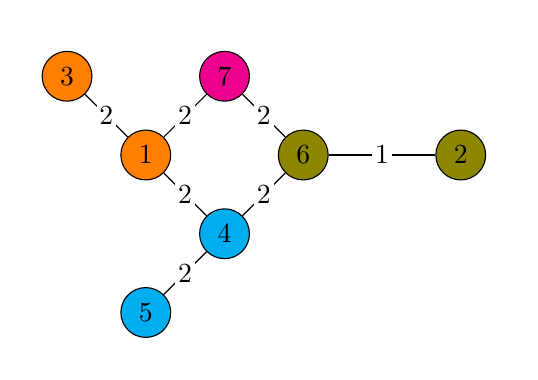
\begin{tikzpicture}
  \fill [white] (-3.5, -2.5) rectangle (2.5, 1.5) node {};  % Zentriere Graph.
  \tikzstyle{node}=[circle,draw, minimum width=18pt, inner sep=0pt, fill=white]
  \tikzstyle{color1}=[fill=orange]
  \tikzstyle{color2}=[fill=olive]
  \tikzstyle{color3}=[fill=cyan]
  \tikzstyle{color4}=[fill=magenta]
  \tikzstyle{label}=[fill=white, inner sep=1pt]

  \node[node, color1] (1) at (-3, 1)  {$3$};
  \node[node, color1] (2) at (-2, 0)  {$1$};
  \node[node, color4] (3) at (-1, 1)  {$7$};
  \node[node, color3] (4) at (-1, -1) {$4$};
  \node[node, color2] (5) at (0, 0)   {$6$};
  \node[node, color3] (6) at (-2, -2) {$5$};
  \node[node, color2] (7) at (2, 0)   {$2$};

  \path (1) edge node[label] {$2$} (2);
  \path (2) edge node[label] {$2$} (3);
  \path (2) edge node[label] {$2$} (4);
  \path (3) edge node[label] {$2$} (5);
  \path (4) edge node[label] {$2$} (5);
  \path (4) edge node[label] {$2$} (6);
  \path (5) edge node[label] {$1$} (7);
\end{tikzpicture}
}
\hspace{1cm}
\subfigure[vergröberter Graph]{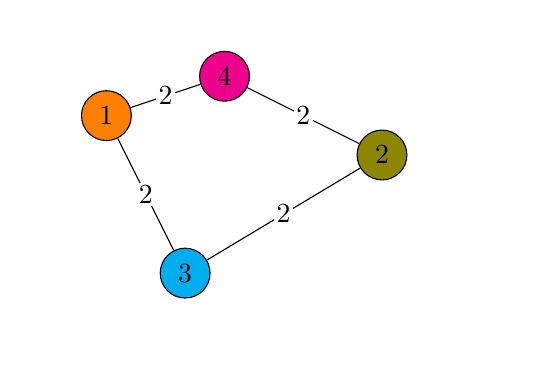
\begin{tikzpicture}
  \fill [white] (-3.5, -2.5) rectangle (2.5, 1.5) node {};  % Zentriere Graph.

  \tikzstyle{node}=[circle,draw, minimum width=18pt, inner sep=0pt, fill=white]
  \tikzstyle{color1}=[fill=orange]
  \tikzstyle{color2}=[fill=olive]
  \tikzstyle{color3}=[fill=cyan]
  \tikzstyle{color4}=[fill=magenta]
  \tikzstyle{label}=[fill=white, inner sep=1pt]

  \node[node, color1] (1) at (-2.5, 0.5)  {$1$};
  \node[node, color2] (2) at (1, 0)       {$2$};
  \node[node, color3] (3) at (-1.5, -1.5) {$3$};
  \node[node, color4] (4) at (-1, 1)      {$4$};

  \path (1) edge node[label] {$2$} (3);
  \path (1) edge node[label] {$2$} (4);
  \path (2) edge node[label] {$2$} (3);
  \path (2) edge node[label] {$2$} (4);
\end{tikzpicture}
}
\caption[Graphvergröberung mittels Graclus und Normalized-Cut]{Vergröberung eines Graphen \gls{G} mittels Graclus und Normalized-Cut bei zufälliger Knotenordung, hier angegeben über die Knotenindizes von \gls{G} (a).
Die Maxima des Normalized-Cuts (b) zwischen den Knoten und deren lokalen Nachbarschaften bestimmen in aufsteigender Reihenfolge das höchstens paarweise Clustering von \gls{V} (c).
Der vergröberte Graph ergibt sich dann als clusterweise Aufsummierung der Kanten ohne Schleifen (d).}
\label{fig:clustering}
\end{figure}
